\chapter{Keeping Information Secret}

The previous chapter \ref{chapter:representing_information_with_symbols} was about representing information with symbols. This section is about keeping information secret.
Ciphers haven been used for thousands of years \cite{HistoryOfCryptography}. They are used to keep information secret from people, that are not supposed to have knowledge of it. Not encrypted information is called clear text. Once one encrypted a clear text, it is called a cipher text and only people who know how to decrypt the cipher text can read originally encrypted information.
The exercises in this section are introducing pupils to the concepts of ciphers.

\section{Cipher Texts from Reversed Letters}

\subsection{Concept}
The cipher used in these exercises is a simple mix up of letters and both directions are trained: encryption and decryption. In the decryption exercise, the pattern, on which the clear text was encrypted with, is shown. The pupils need to understand the pattern and move the letters in the cipher text accordingly to retrieve the clear text. The encryption exercise is set up analogously. Multiple difficulty levels are possible by changing the amount of moved letters.

\begin{example}
    The cipher text is \code{ULFSS} and the pattern is shown in figure \ref{fig:pattern}. By moving the letter in the cipher text according to the pattern, the clear text can be retrieved: \code{FLUSS}.
\end{example}

\begin{figure} 
    \centering
    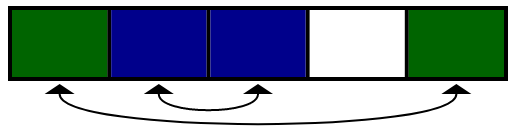
\includegraphics[width=0.4 \columnwidth]{figures/pattern.png}
    \caption{Pattern} 
    \label{fig:pattern} 
\end{figure}

\subsection{Implementation}

\section{Cipher Texts from New Characters}

\subsection{Concept}
Sometimes, only moving symbols in not enough to keep information secret. A better why is to substitute symbols with new symbols. These symbols may be letters, numbers or completly new symbols, that are solely invented for the purpose of encrypting information.
In the following exercises the last approach is followed. Again both direction, encryption and decryption, are trained. But this time, instead of having a pattern, there is a symbol table showing how the letters are encrypted. 

\begin{example}
    The cipher text is shown in figure \ref{fig:cipher_number} and the symbol table in figure \ref{fig:symbol_table}. By using the symbol table one can decrypt the cipher text to \code{52}.
\end{example}

\begin{figure} 
    \centering
    
\includegraphics[width=0.2 \columnwidth]{figures/cipher_number.png}
    \caption{Cipher text of an encrypted number} 
    \label{fig:cipher_number} 
\end{figure}

\begin{figure} 
    \centering
    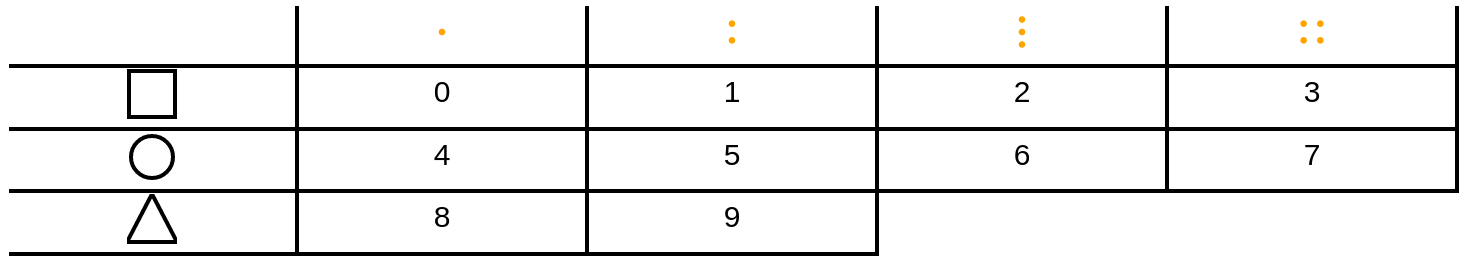
\includegraphics[width=1.0 \columnwidth]{figures/symbol_table.png}
    \caption{Symbol table to encrypt numbers} 
    \label{fig:symbol_table} 
\end{figure}

\subsection{Implementation}
% drawing on canvas